\section{Overview} 

\begin{figure}[H]
    \centering
    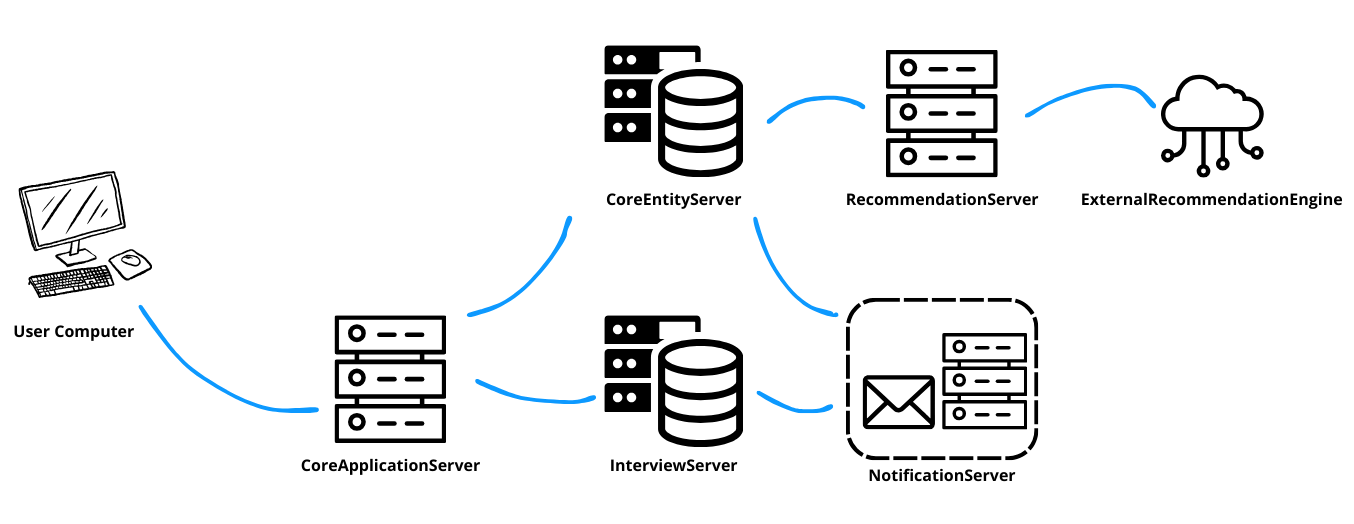
\includegraphics[width=\textwidth]{Images/informal-view.png}
    \caption{Informal View of the System}
    \label{fig:informal_view}
\end{figure}

The informal view of the system provides a high-level representation of the key components and their interactions within the Students\&Companies (S\&C) platform. The design prioritizes modularity, scalability, and maintainability, reflecting the architectural decisions made to address the platform's requirements effectively.

A microservices architecture forms the foundation of the system, enabling decoupled services to interact through well-defined interfaces. This design choice ensures that individual components, such as authentication, matchmaking, and notifications, can be developed, deployed, and scaled independently. Communication between these components is facilitated through secure RESTful APIs and asynchronous messaging systems, enhancing fault tolerance and performance.

By abstracting critical elements like the RecommendationEngine as a black-box component, the design provides flexibility for future updates or replacements without disrupting other parts of the system. Furthermore, distributed databases ensure data consistency and fault isolation, allowing the platform to handle a diverse range of user interactions efficiently.


\section{Component view}

As mentioned, the chosen architecture is a microservice architecture, in which the components are abstracted to include a decoupled service and they interact with each other with well defined interfaces to request for each others different competences. The component view can be seen at \ref{fig:component_diagram} and describes the following components:
\begin{itemize}
    \item \textbf{AuthenticationService} provides the authentication of user credentials
    \item \textbf{Main Platform} routes the API calls from the FrontEndInterface to other components with respective databases and services, also takes part in coordination in some use cases.
    \item \textbf{FrontEndInterface} is the graphic user interface available to the user through Web
    \item \textbf{HistoryManager} is responsible for storing and maintaining complaints and feedbacks of users.
    \item \textbf{CoreEntityManager} is responsible for storing, mantaining and giving functionality to some core entities, such as internships, students, applications, etc.
    \item \textbf{InterviewManager} is strictly responsible to store, maintain and give the functionalities of interview, including start it, finish it, assess its handling by the company user etc.
    \item \textbf{RecommendationScheduler} is responsible to periodically scan for reccomendations and coordinate the handling of the recommendation engine
    \item \textbf{DataProcessor} is responsible to assess RecommendationScheduler and CoreEntityManager on the data cleaning and pre processing to send to the RecommendationEngine
    \item \textbf{RecomendationEngine} models the external cloud tool to generate recommendations for internships and students
    \item \textbf{NotificationListener} is responsible of taking in messages of entities that wish to send notifications to actors
    \item \textbf{NotificationDispatcher} is responsible to receive the notification requests and dispatch it to the users through a mailing service, also includes in its internal logic choices as in how often to email etc.

    
    
\end{itemize}

\begin{figure}[H]
    \centering
    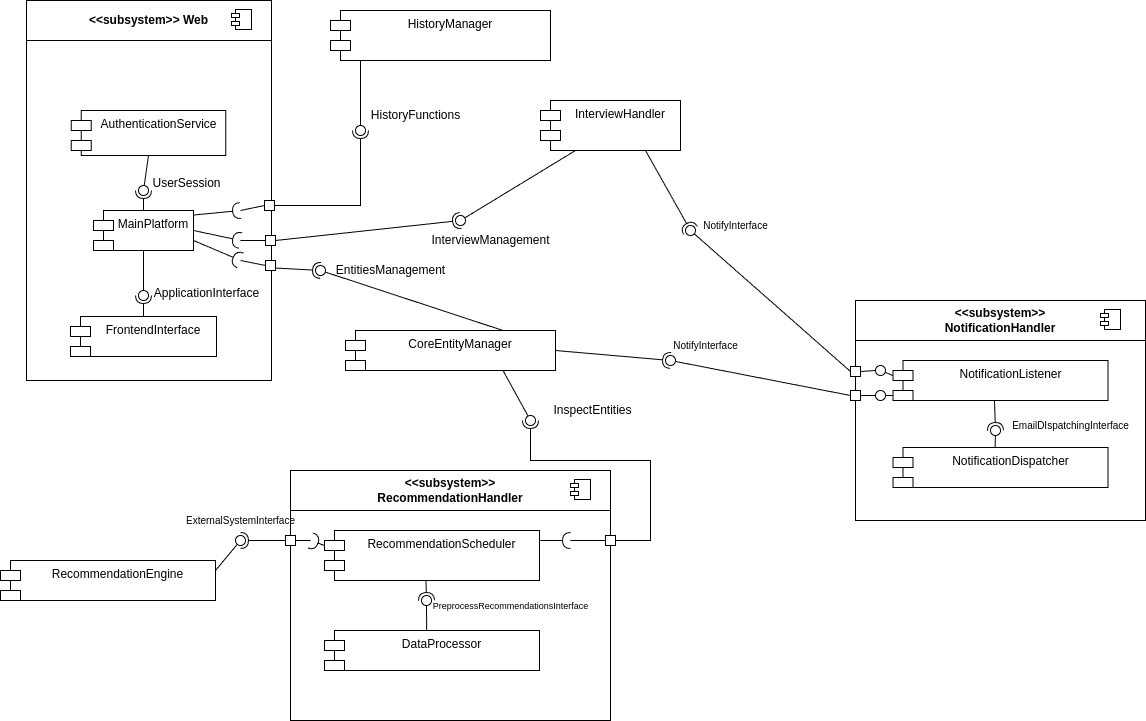
\includegraphics[width=\textwidth]{Images/component-view.png}
    \caption{Component Diagram}
    \label{fig:component_diagram}
\end{figure}

\section{Deployment view}

Here is shown the deployment view diagram, which is important because it illustrates the physical layout of the system, showing how software components are deployed onto hardware nodes. This view is essential for understanding system scalability, fault tolerance, and performance optimization by highlighting the relationships and communication paths between components. It can be seen on figure \ref{fig:deployment_diagram}.

\begin{figure}[H]
    \centering
    \rotatebox{90}{
        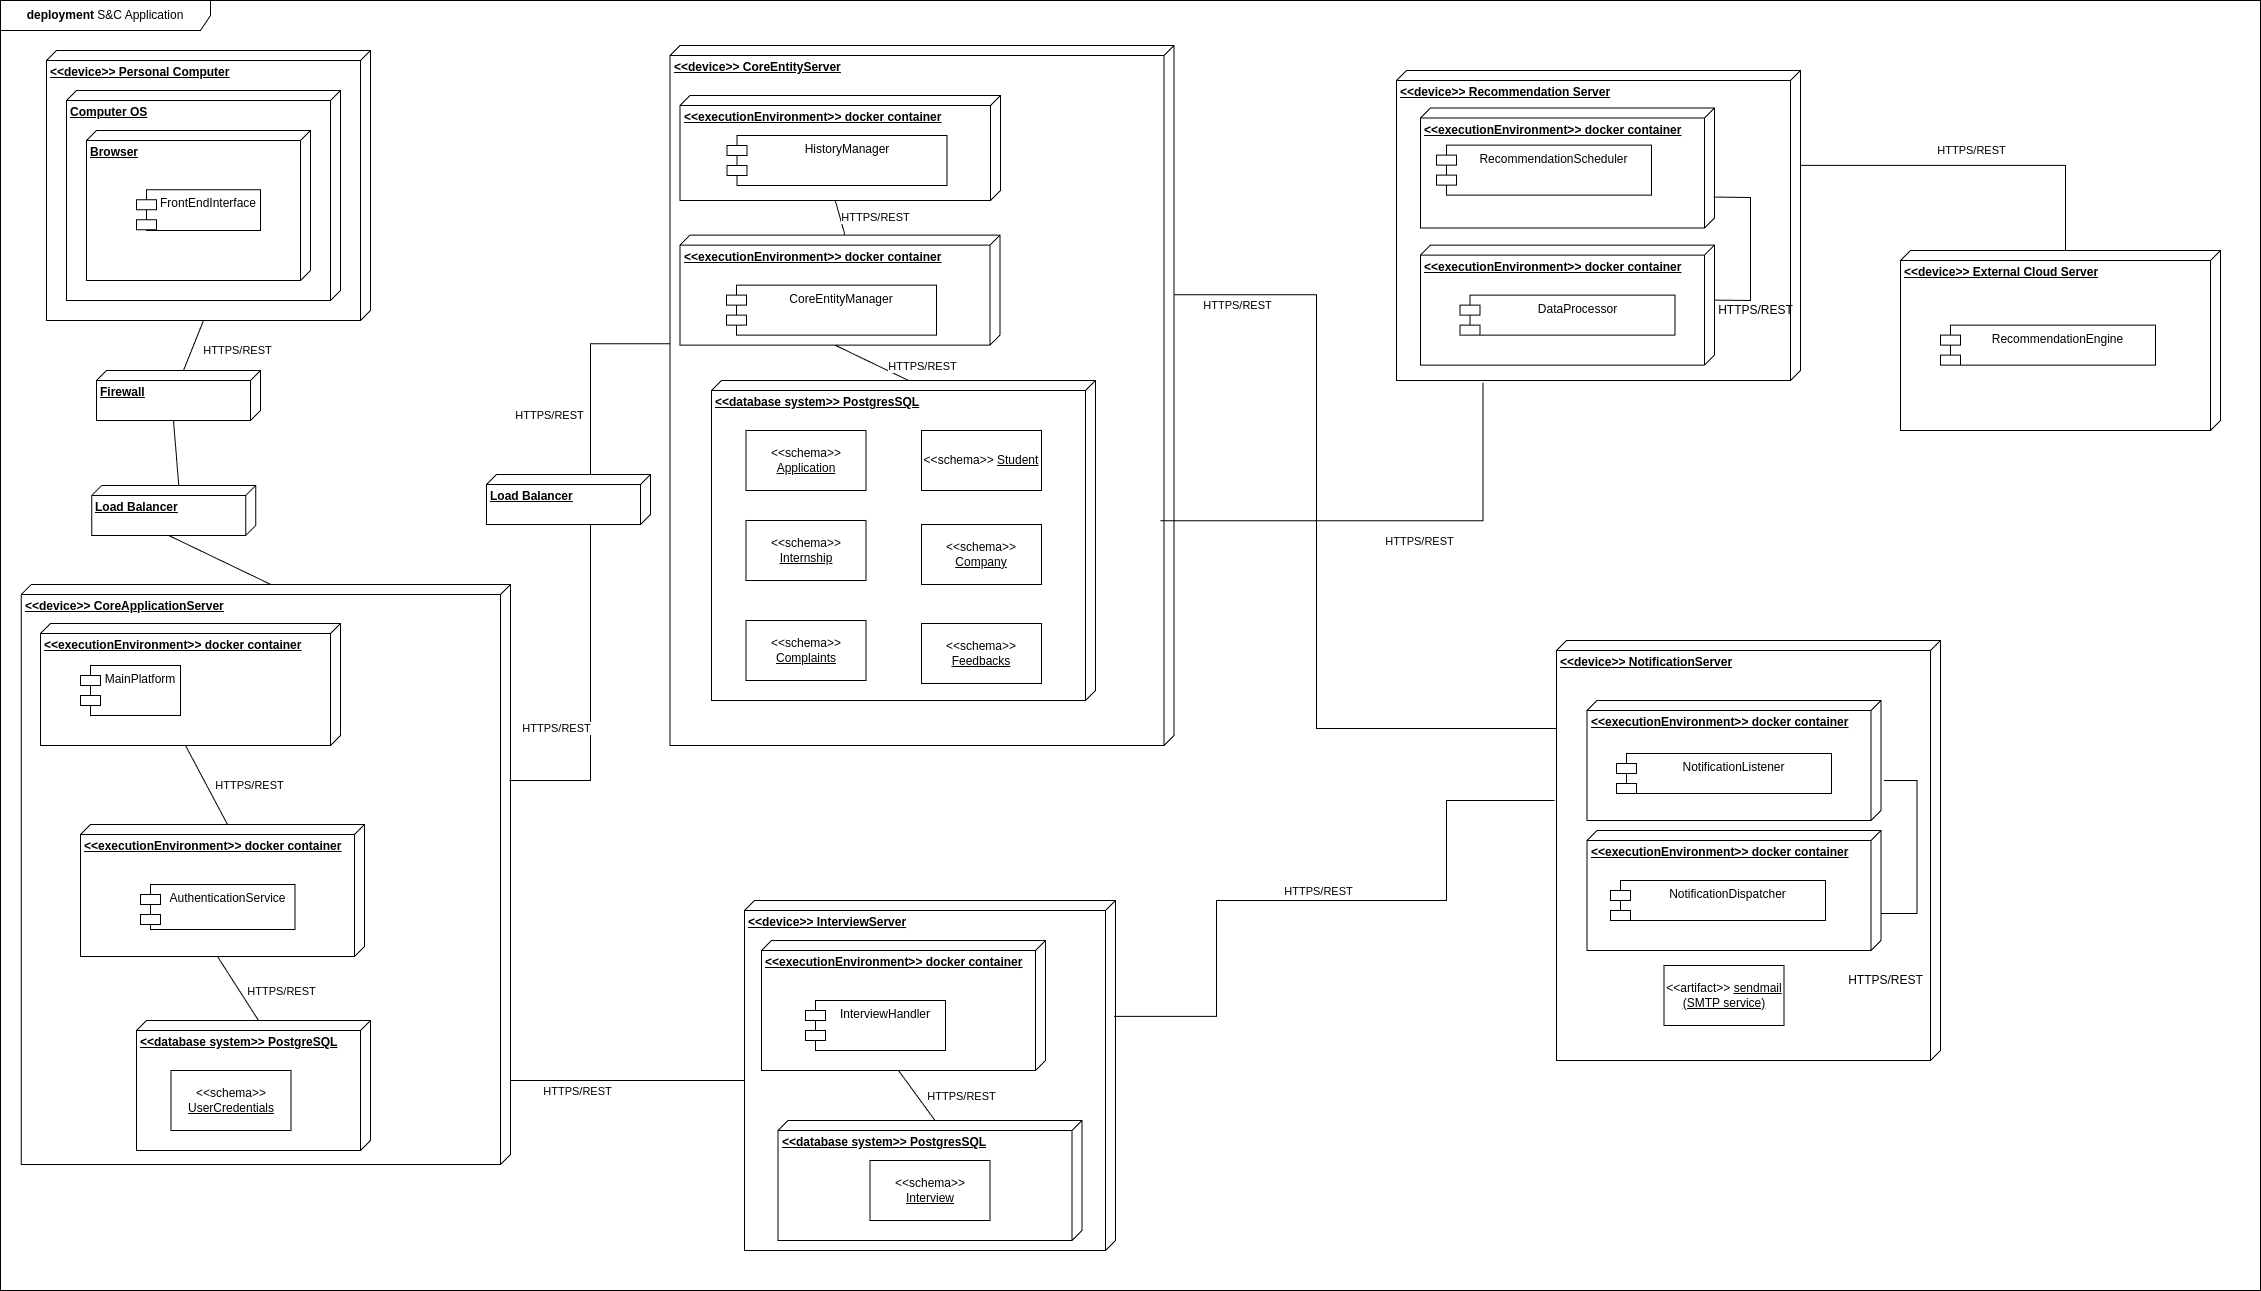
\includegraphics[width=0.9\textheight]{Images/deployment-view.png}
    }
    \caption{Specification Level Deployment Diagram}
    \label{fig:deployment_diagram}
\end{figure}

In \ref{fig:deployment_diagram} it can be seen that the microservices architecture allows a distributed implementation onto hardware which can be exploited also for replication and optimization, achieving reliabilty, safety and secureness, and fault tolerance.
The components are all abstracted on a docker container so that the system is portable and the architecture can change without major firmware issues. Also, the components are grouped in different servers according to functionality and frequency of communication.

The LoadBalancers guarantee that replicated critical servers and components have a reasonably equal workload among them, and the firewall protects against attacks comming from the FrontEndInterface, which is runned on the browser of the user and therefore we have less control of. The NotificationServer also includes a mailing system so that the NotificationDispatcher can send emails via SMTP, and the RecommendationEngine is modelled as an external server running on a cloud solution. 

All servers communicate through HTTPS/REST API calls defined internally on the system, except the RecommendationEngine that is defined by the solution itself, but the RecommendationServer components adress this internally.

\section{Runtime view}

This section introduces the runtime view of the system, that is, its dynamic behavior across use cases. The 4 use cases that were documented on the RASD with sequence diagrams also have their sequence diagrams here for coherence with the RASD, while the other simpler ones are explained textually.

\textbf{[UC1] Form Filling}

The user fills the empty form on the FrontEndInterface and submits it. The FrontEndInterface sends the data to the MainPlatform, which runs its validation logic. In case of validation failure, an error is returned to the FrontEndInterface for user correction. Here, the MainPlatform can apply some other procedures on the data (for example, send it to other component for storage). Finally, the MainPlatform sends an ``OK'' back to the FrontEndInterface, which displays a success message.


\textbf{[UC2] Register Student}

The student opens the S\&C Website via the FrontEndInterface and clicks ``New Account''. The FrontEndInterface requests a registration form from the MainPlatform, which calls the AuthenticationService to validate and store the new user’s credentials. Meanwhile, any additional profile information is passed from the MainPlatform to the CoreEntityManager for storage. Once validation succeeds, both the AuthenticationService and CoreEntityManager send ``OK'' back to the MainPlatform, which then notifies the FrontEndInterface. Finally, the FrontEndInterface displays a confirmation that the student’s account is successfully registered.

\textbf{[UC3] Register Company}

The company employee opens the S\&C Website via the FrontEndInterface and clicks ``New Account''. The FrontEndInterface requests a registration form from the MainPlatform, which calls the AuthenticationService to validate and store the new company account credentials (email, password). Meanwhile, any additional company data (e.g., name, industry) is passed from the MainPlatform to the CoreEntityManager for storage. Once both the AuthenticationService and CoreEntityManager send an ``OK'' back to the MainPlatform, the MainPlatform notifies the FrontEndInterface. Finally, the FrontEndInterface displays a confirmation that the company account has been successfully created.

\textbf{[UC4] User Login}

The user opens the S\&C Website on the FrontEndInterface and clicks ``Log In''. The FrontEndInterface sends the entered email and password to the MainPlatform, which calls the AuthenticationService to check the credentials. If valid, the AuthenticationService confirms, and the MainPlatform creates a user session. It then notifies the FrontEndInterface, which displays the user’s dashboard. If invalid, the MainPlatform returns an error message, leading the FrontEndInterface to prompt the user to retry.


\textbf{[UC5] Search Internship} (Figure \ref{fig:searchsequence})
\begin{figure}[H]
\centering
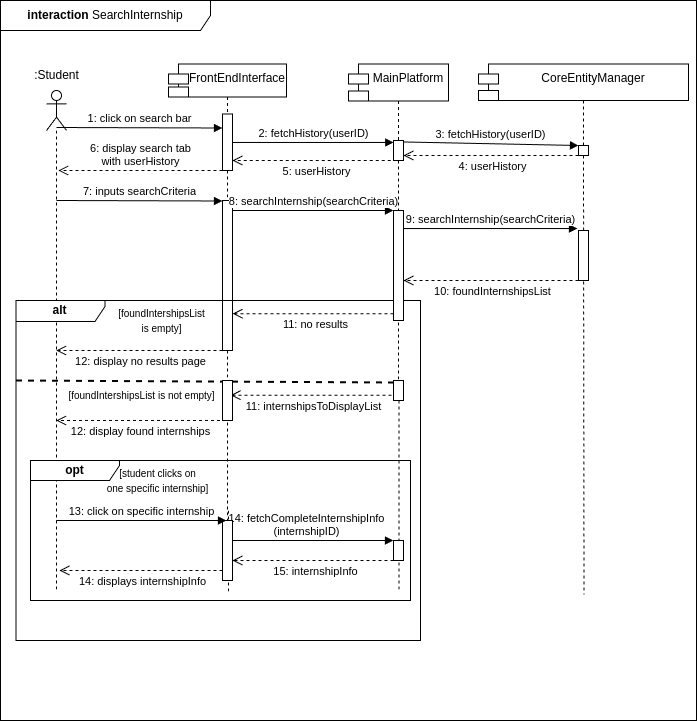
\includegraphics[width=\textwidth]{Images/search-internship-sequence.png}
\caption{\label{fig:searchsequence} Search Internship Sequence Diagram}
\end{figure}


The process is started when a Student clicks on the Search Bar once in the main page, which makes the FrontEndInterface fetch the userHistory of that user to display the beneath the search bar. With the history displayed, the Student inputs the desired search criteria on the FrontEndInterface or picks from his recent history, which passes it to the MainPlatform, that also passes it to the CoreEntityManager. This component then looks up on its internal database and passes back to the MainPlatform, which returns with either a ``no result'' to the FrontEndInterface or the list of found internships, depending on this list being empty or not.

Once the results are showed, if any, the student may click on a specific internship, causing the FrontEndInterface to fetch the remaining information of the internship from the MainPlatform (cached after the first fetch) and, after response, the user can see it.

\textbf{[UC6] Apply Internship}

The student, already logged in, views the internship details through the FrontEndInterface. When they click the ``Apply'' button, the FrontEndInterface sends the application request to the MainPlatform, which recognizes the active user session. The MainPlatform then forwards this request to the CoreEntityManager to record the application. Once saved, the CoreEntityManager confirms back to the MainPlatform, which returns a success status to the FrontEndInterface. Finally, the FrontEndInterface displays an ``Application Successful'' page and informs the student about the expected feedback timeframe.


\textbf{[UC7] New Recommendation} (Figure \ref{fig:matchmakingseq})

% \begin{figure}[H]
%     \centering
%     \rotatebox{90}{
%         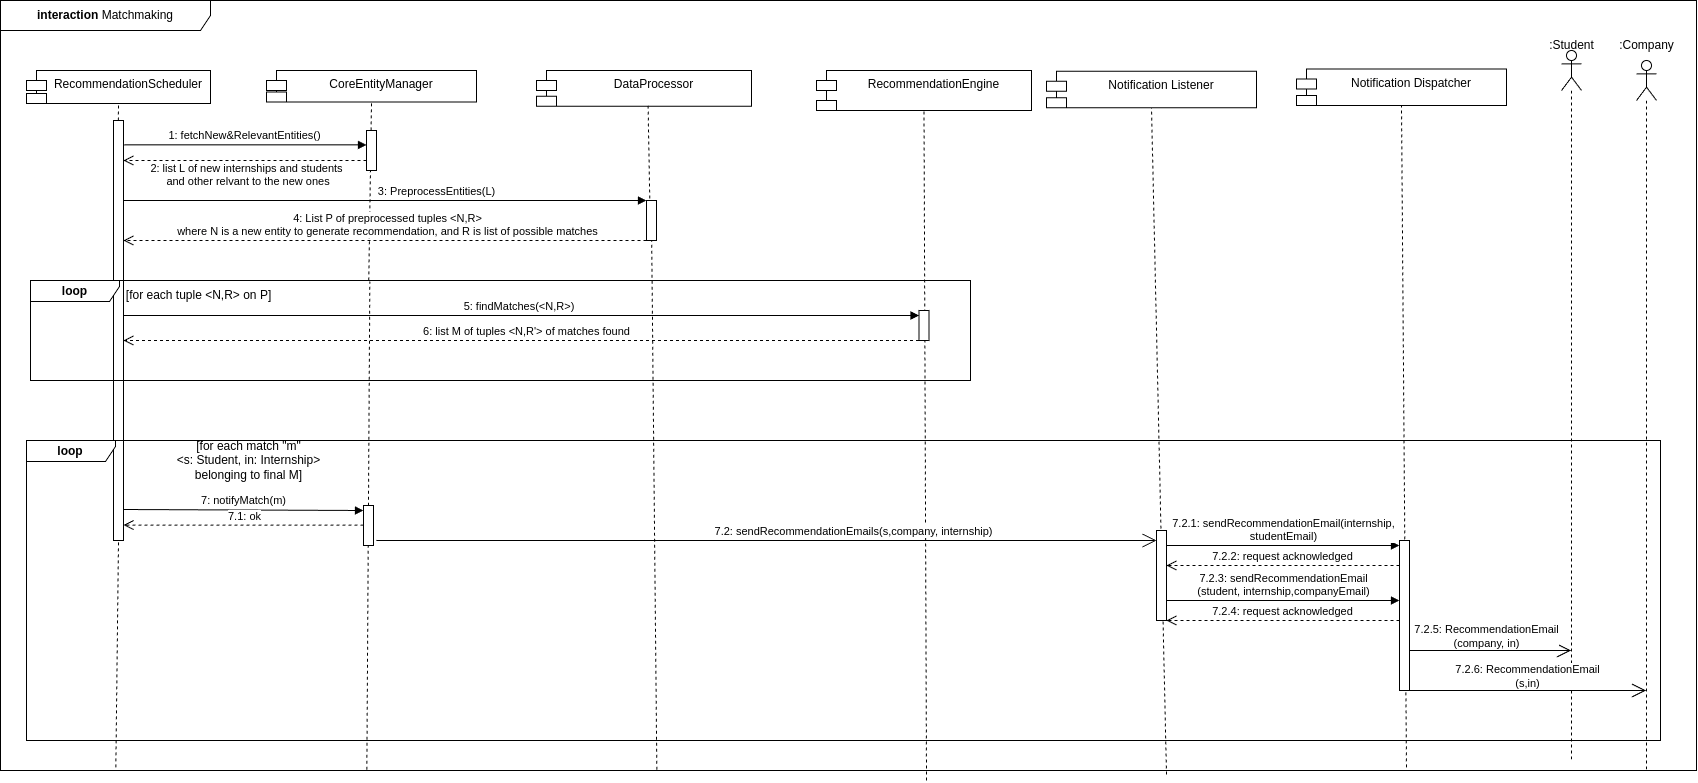
\includegraphics[width=0.9\textheight]{Images/matchmaking-process-sequence.png}
%     }
%     \caption{New Recommendation Sequence Diagram}
%     \label{fig:matchmakingseq}
% \end{figure}

\begin{figure}[H]
\centering
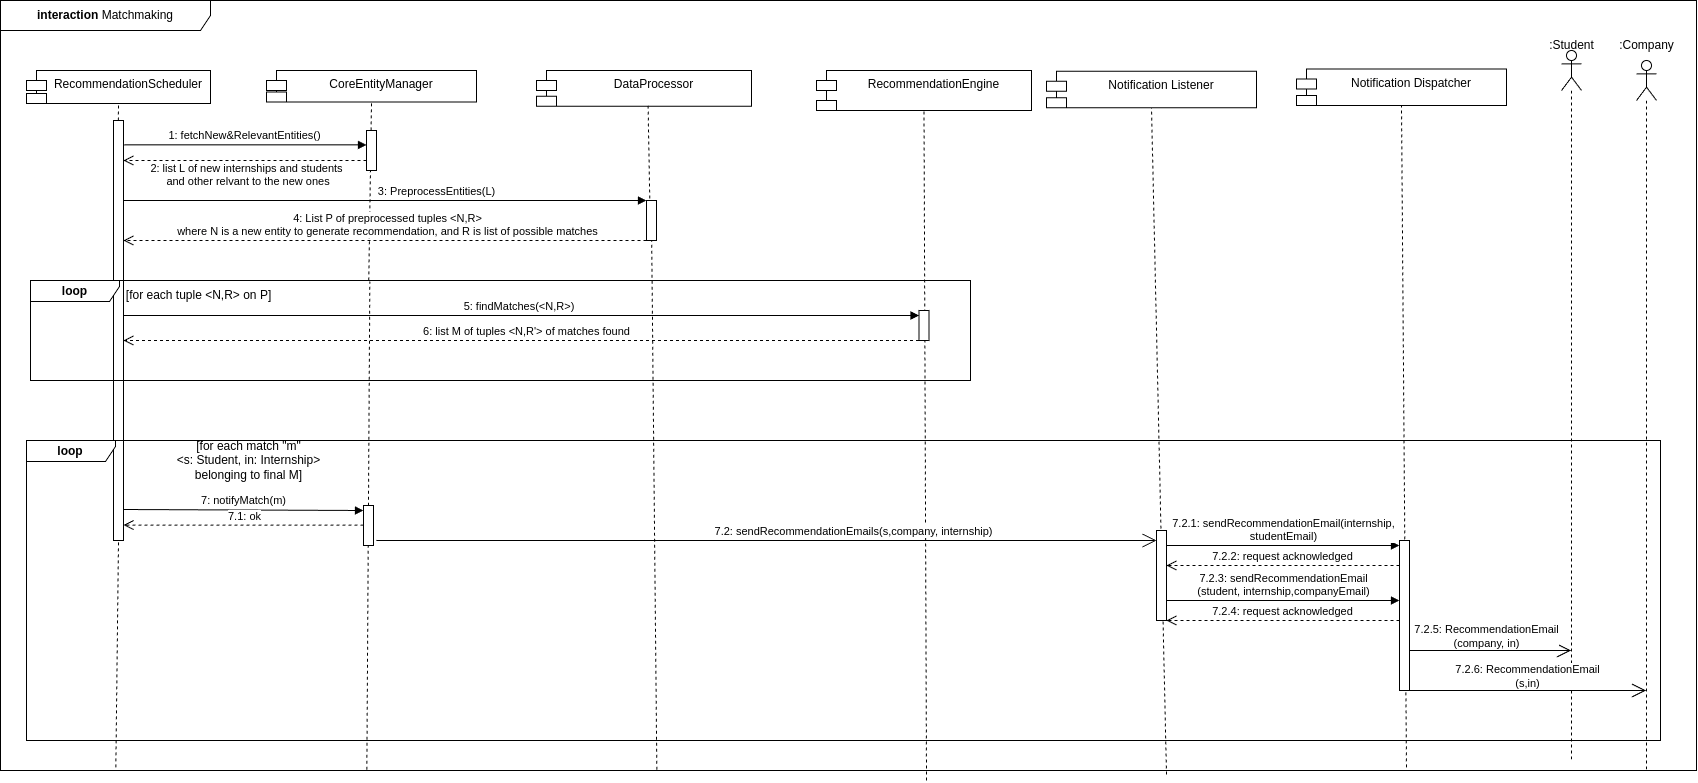
\includegraphics[width=\textwidth]{Images/matchmaking-process-sequence.png}
\caption{\label{fig:matchmakingseq} New Recommendation Sequence Diagram}
\end{figure}

The process begins with the RecommendationScheduler invoking fetchNew\&RelevantEntities() method on the CoreEntityManager (this is scheduled as a CronJob process on the server's OS and is fired regularly). This retrieves a list (L) of newly added internships and students, as well as entities relevant to them according to hard filters (such as the candidate's refusal to move country, for example). 

Once all the new and relevant students and internships are returned to RecommendationScheduler, it calls the DataProcessor to preprocess these entitites. The DataProcessor now generates a structured list P of tuples <N,R> where each N is a new internship or student and R is a list of all relevant counterparts to it. Now, with data structured in a way the RecommendationEngine can understand it, the RecommendationScheduler sends  the tuples one by one to the RecommendationEngine, that returns a list M of tuples of recommended matches based on its internal algorithm.

Now, to send the notifications, for each tuple <N, R> in M, notify the CoreEntity manager through notifcyMatch(n), which in turn will send a message to the NotificationListener, that passes this on to the NotificationDispatcher, which fires all recomenddation emails once they are gathered and its internal algorithm decides to (for example, the company's emails may be buffered until many recommendations are reached, or sent every week, etc.).


\textbf{[UC8] New Internship}

The company employee, already logged in, clicks ``New Internship Position'' on the FrontEndInterface. The FrontEndInterface retrieves the form from the MainPlatform, which displays fields for the internship details (name, requirements, duration, etc.). After the company employee completes and submits the form (included use case: form filling), the MainPlatform passes the new internship information to the CoreEntityManager for storage. Once successfully stored, the CoreEntityManager returns an ``OK'' to the MainPlatform, which confirms with the FrontEndInterface that the position is created. The FrontEndInterface then displays to the company employee that the internship position is now published.

\textbf{[UC9] Cancel Internship}

The company employee, already logged in, opens ``Open Internships'' on the FrontEndInterface. The MainPlatform fetches the list of open internships from the CoreEntityManager, which returns them for display. When the employee chooses an internship to cancel and clicks ``Cancel Internship,'' the FrontEndInterface sends this request to the MainPlatform. The MainPlatform passes the cancellation to the CoreEntityManager, which updates the internship’s state to ``cancelled''. Because of this state change, the internship no longer appears in searches or recommendations. The CoreEntityManager then notifies the MainPlatform, which confirms the cancellation to the FrontEndInterface, displaying to the company's actor that the internship was successfully canceled.

\textbf{[UC10] Schedule Interview} (Figure \ref{fig:schedulesequence})
\begin{figure}[H]
\centering
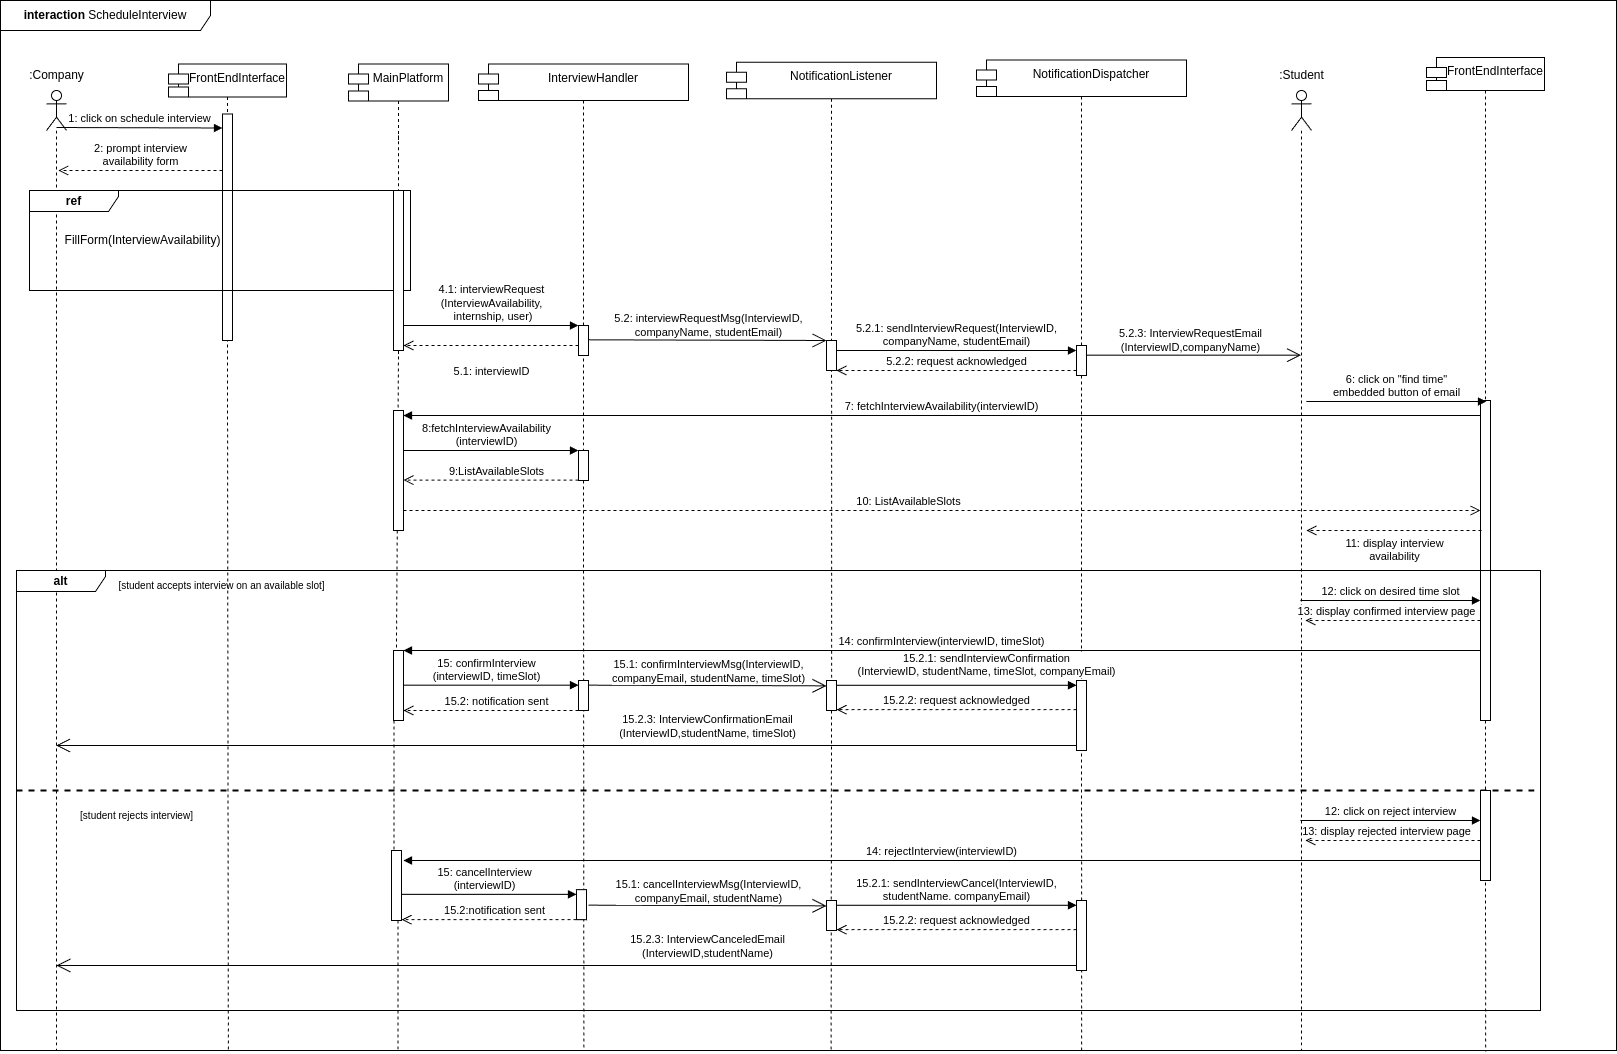
\includegraphics[width=\textwidth]{Images/schedule-interview-sequence.png}
\caption{\label{fig:schedulesequence} Schedule Interview Sequence Diagram}
\end{figure}


The process is started when a Company actor clicks on the "schedule interview" , which makes the FrontEndInterface prompt an availability form for the company agent to fill with the available date and time, the filled answers on the FrontEndInterface are passed to the MainPlatform, that also passes it to the Interview Handler, which creates the interview and returns an ID. This component also starts the notification process sending a message to the NotificationListener, which ends with the Student getting an email.

Once Student clicks on the "find time" button on the email, they are redirected to the S\&C page and another instance of FrontEndInterface starts running on the browser, which fetches the interview availability from the MainPlatform to list the available slots to the Student, which also involves the MainPlatform getting back from the InterviewHandler the availability of the stored interview.

With the availability displayed to the Student, they may either choose a Slot or reject the Interview. In the first case scenario, the FrontEndInterface passes the confirmation to the MainPlatform, which then passes it to the InterviewHandler so the state of the interview is changed and a notification sent to the company's email with a confirmation of date and time for the interview. If, instead, the Student rejects the interview, the same process happens but with rejection messages and the logic inside the InterviewHandler changes.

\textbf{[UC11] Process Interview}
(Figure \ref{fig:processinterviewsequence})
\begin{figure}[H]
\centering
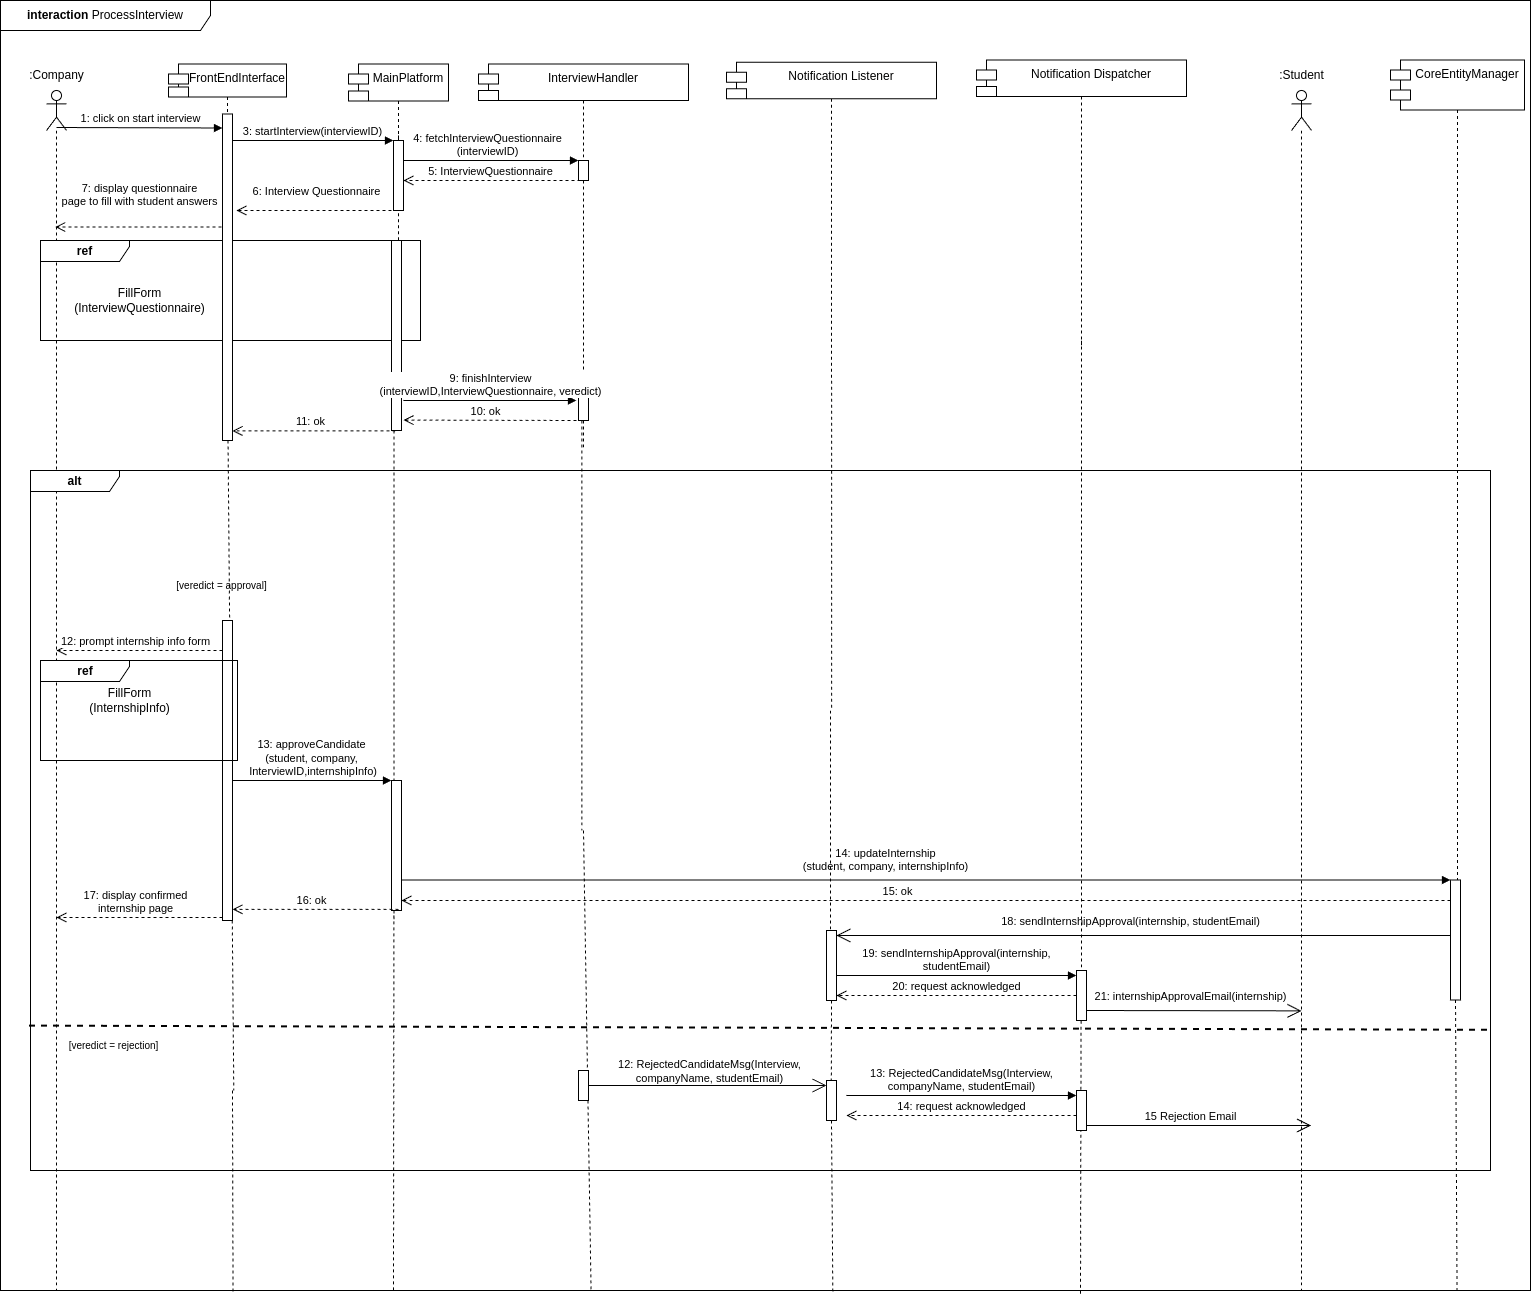
\includegraphics[width=\textwidth]{Images/interview_process-sequence.png}
\caption{\label{fig:processinterviewsequence} Process Interview Sequence Diagram}
\end{figure}

The process is started when a Company actor clicks on the "start interview" , which makes the FrontEndInterface pass this to the MainPlatform as a request for the form to be filled during the interview. The MainPlatform then fetches the form from the InterviewHandler through the interviewID, and the form is passed all the way back to the Company through the display on the FrontEndInterface. Once the form is filled, the interview is finished with a filled form and a veredict, both of which the FrontEndInterface passes to the MainPlatform so it can pass to the InterviewHandler to update the interview status. With the status saved, S\&C proceeds to process the result and notify the student.

If the veredict is true, the FrontEndInterface uses the internship info form (with information wuch as start date, place, etc.) and prompts it to the Company's actor. When it's filled, this component passes the internship information to the CoreEntityManager so it can alter its status and information. Once done with its internal logic, it sends triggers the email notification process by sending a message to the NotificationListener.

In the case of the veredict being false, the only further action needed is to notify the Student since the InterviewHandler already got the veredict and processed it internally, so this component is the one to trigger the notification process by senidng a message to the NotificationListener.


\textbf{[UC12] New Complaint}

The user, already logged in, navigates to ``Ongoing Internships'' on the FrontEndInterface. The FrontEndInterface requests the list of internships from the MainPlatform, which in turn fetches them from the CoreEntityManager and displays them. The user selects the relevant internship and clicks ``Create Complaint,'' triggering the complaint form (included use case: form filling). Once submitted, the FrontEndInterface sends the complaint data to the MainPlatform, which forwards it to the HistoryManager (responsible for feedback, complaints, and analytics). The HistoryManager stores the complaint in the internal database and returns an ``OK'' to the MainPlatform, which confirms success to the FrontEndInterface.


\textbf{[UC13] Post Internship Feedback}

With the user in the ``Provide Feedback'' page of a given closed internship, The FrontEndInterface then displays a feedback form (included use case: form filling). After submission, it sends the feedback data to the MainPlatform, which forwards it to the HistoryManager for storage and calls the CoreEntityManager to update the internship’s status. Finally, the CoreEntityManager triggers a notification handled by the NotificationListener and later passed on to the NotificationDispatcher, alerting the other party (student or company) that the feedback has been submitted.



\section{Component interfaces}

This section introduces every interface of the modeled components, so that the runtime behavior described previously can be understood in a component-level abstraction and to aid the developer on their implementation.

\subsubsection{FrontEndInterface} 


This component offers no interfaces since it is, in itself, a visual interface to the user that interact via web browsing.




\subsubsection{MainPlatform} 

This component offers only one interface, \textbf{ApplicationInterface}
which is offered to the FrontEndInterface:
\begin{itemize}
    \item \texttt{submitForm(formData)} 
    Sends form data from the frontend to be processed.
    \item \texttt{requestStudentRegistration(regData)} Initiates a student registration request.
    \item \texttt{requestCompanyRegistration(regData)} Initiates a company registration request.
    \item \texttt{login(email, password)} Captures user credentials and forwards them for authentication.
    \item \texttt{applyToInternship(internshipId)} Sends the student’s application request for a specific internship.
    \item \texttt{createInternship(data)} Submits new internship details for creation.
    \item \texttt{viewOpenInternships(companyID)} Requests the list of open internships for a given company.
    \item \texttt{cancelInternship(internshipId)}
    \item \texttt{fetchHistory(userID)}
    This is used to fetch the user search history, returning it as a list of performed searches.
    \item \texttt{searchInternship(searchCriteria)}
    This is used to pass the searchCriteria to the CoreEntityManager to perform the search on its database, it returns either a "no results" message or a list of internships to display
    \item \texttt{fetchCompleteInternshipInfo(internshipID)}
    This is used to fetch the complete information about an specific internship (the FrontEndInterface uses it after the User clicks on a specific internship). It returns the internshipInfo.
    \item \texttt{finishInterview(interviewID, interviewQuestionnaire, veredict)}
    This is used so that the FrontEndInterface indicates that the interview with interviewID is finished and the provided information is composed of the filled interviewQuestionnaire and the veredict upon the interview. This is passed on to the interviewHandler and returns just an "ok" message to indicate everything worked out fine.
    \item \texttt{fileComplaint(internshipId, complaint)} Submits a complaint for a specific internship.
    \item \texttt{submitFeedback(internshipId, feedback)} Sends user feedback about a specific internship.
\end{itemize}



\subsubsection{AuthenticationService}

This component offers only one interface, \textbf{UserSession}, which is offered to the MainPlatform:
\begin{itemize}
    \item \texttt{createAccount(email, password)} Creates a new user account.
    \item \texttt{authenticate(email, password)} Validates credentials.
\end{itemize}



\subsubsection{CoreEntityManager}
This component offers two different interfaces.

\textbf{InspectEntities} is offered to the RecommendationScheduler:
\begin{itemize}
    \item \texttt{fetchNewAndRelevantEntities()}
    This is used to fetch all the new entities and the ones relevant to those new ones in terms of matchmaking. It triggers an access to the database, as well as some internal logic to apply the hard filters specified on the newly fetched entities(e.g. a student refusal to move country) to define the "relevant" ones to be searched. It returns a list of found internhsips and students, both new or relevant.
    \item \texttt{notifyMatch(m: <s:Student, in: Internship>)}
    This is used to notify the component that a match has been found between `in` and `s`. This activates the internal match dealing logic of CoreEntityManager and triggers the email-sending process to both parts.
\end{itemize}

\textbf{EntitiesManagement} is offered to the MainPlatform:
\begin{itemize}
    \item \texttt{storeData(formData)} Saves the form data into the internal storage.
    \item \texttt{storeStudentProfile(userID, workProfile)} Stores the student’s work profile information.
    \item \texttt{storeCompanyProfile(userID, compProfile)} Stores the company’s profile information.
    \item \texttt{createApplication(userId: int, internshipId: int)} Logs the application entry into the system.
    \item \texttt{searchInternship(searchCriteria)}
    This inputs the searchCriteria specified by the user and triggers an access to its internal database. It returns a list of found internships
    \item \texttt{storeInternship(data)} Persists the new internship information to storage.
    \item \texttt{fetchInternships(companyID, state?)} Retrieves internships by company and (optionally) state.
    \item \texttt{updateInternshipState(internshipId, newState)} Changes the internship’s state.
\end{itemize}



\subsubsection{InterviewHandler}
This component offers only one interface, \textbf{InterviewManagement}, which is offered to the MainPlatform
\begin{itemize}
    \item \texttt{interviewRequest(interviewAvailability, internship, user)}
    This is used to request a new interview, leading to the instancing of a interview entity and altering the database records. It also triggers a notification message to the Notification Listener so that the Student gets an email about the attemptive interview. It returns the interviewID of the newly instanced interview.
    \item \texttt{fetchInterviewAvailability(interviewID)}
    This is used to consult the availability of an existing interview, instanced through the previous documented call. It returns the interview availability, which is just a list of the available time slots.
    \item \texttt{confirmInterview(interviewID, timeSlot)}
    This is used to confirm an attemptive interview with interviewID in a given timeSlot. Besides internally changing its state, it triggers the notification process by sending a message to NotificationListener so that the Company is notified about the time of the interview. It returns a "notifcation sent" message just meaning everything worked ok.
    \item \texttt{cancelInterview(interviewID)}
    This is used to cancel an attemptive interview with interviewID. Besided internally changing the state of the interview, it sends a message to NotificationListener, so that the Student also gets an email about its cancellation. It also returns a "notifcation sent" message just meaning everything worked ok.
    \item \texttt{fetchInterviewQuestionnaire(interviewID)}
    This is used to get the stored interview questionnaire for the internship corresponding to the interview of interviewID. It returns the requested questionnaire which is only a form.
    \item \texttt{finishInterview(interviewID, interviewQuestionnaire, veredict)}
    This is used to finish an ongoing interview of ID interviewID. It alters the internal state of the interview, saves the provided information and returns an "ok" message to indicate everything worked out fine.
\end{itemize}


\subsubsection{HistoryManager} 

This component offers one interface, \textbf{HistoryFunctions}, which is offered to the Main Platform:
\begin{itemize}
    \item \texttt{saveComplaint(complaint)} Saves the complaint details into the database.
    \item \texttt{saveFeedback(feedback)} Saves the feedback details into the database.
\end{itemize}


\subsubsection{RecommendatonScheduler} 

This component offers no interfaces, since it is only activated regularly through a CronJob scheduled process on its server OS and only uses other interfaces.


\subsubsection{DataProcessor} 

This component offers only one interface, \textbf{PreprocessRecommendationsInterface}, which is offered to the RecommendationScheduler
\begin{itemize}
    \item \texttt{PreprocessEntities(L)} This triggers the component's internal logic of separating the list into tuples <N,R> of new and "relevant to the new" entities, respectively. It returns a list P of such tuples in a format compatible with the RecommendationEngine provided interface ExternalSystemInterface.
\end{itemize}

\subsubsection{RecommendationEngine} 

This component offers only one interface, \textbf{ExternalSystemInterface}, which is offered to the RecommendationScheduler and would depend on the used external system. It is only assumed it can handle one function call to generate matches, and the specific format of input or output can be adjusted on the DataProcessor internals so it is compatible with the used system.
\begin{itemize}
    \item \texttt{findMatches(<N: new entity to generate recommendation for, R: list of relevant entities to N, from which to decide on recommendations>)} This returns a list of tuples <N,R'> of each match found (R' is only one instance of entity, while R is a list).
\end{itemize}

\subsubsection{NotificationListener} 

This component offers only one interface, \textbf{NotifyInterface}, which is used by both InterviewHandler and CoreEntityManager. Each  message only differs in behaviour on the information input, which one of the two entities sends it and which further message is passed on the NotificationDispatcher, to indicate different email formats. They dont't return anything since it is an asynchronous message.
\begin{itemize}
    \item \texttt{interviewRequestMsg(InterviewID, companyName, studentEmail)}
    This is sent by the InterviewManager and triggers a call to sendInterviewRequest()
    \item \texttt{confirmInterviewMsg(InterviewID, companyEmail, studentName, timeSlot)}
    This is sent by the InterviewHandler and triggers a call to sendInterviewConfirmation()
    \item \texttt{cancelInterviewMsg(interviewID, companyEmail, studentName)}
    This is sent by the InterviewHandler and triggers a call to sendInterviewCancel()
    \item \texttt{sendRecommendationEmails(s: Student, company, internship)} This is sent by the CoreEntityManager and triggers two calls to \texttt{sendRecommendationEmail()} to the NotificationDispatcher, one with internship and studentEmail (that will send an email to the student) and the other with the student, internship and companyEmail (that will send an email to the company).
    \item \texttt{RejectedCandidateMsg(Interview, companyName, studentEmail)}
    This is sent by the InterviewHandler and triggers a call to RejectedCandidateMsg() on the NotificationDispatcher interface
    \item \texttt{sendInternshipApproval(internship, studentEmail)}
    This is sent by the CoreEntityManager and triggers a call to sendInternshipApproval() on NotificationDispatches interface
    \item \texttt{sendFeedback(internship, email)}
\end{itemize}


\subsubsection{NotificationDispatcher}
This component offers only one interface, \textbf{EmailDispatchingInterface}, which is offered to the NotificationListener. All function calls on this interface are to request an email to be sent as notification and it always returns a "request acknowledged" message (before the actual email is sent) just to note that the request has arrived properly and the email will be processed. The interface could be defined as only one \texttt{sendEmail(recipient, subject, body)} function, but here it is also specified some of the different forms of emails that may be called from other entities that want a pre-formatted email to be sent without dealing with what that format is.
\begin{itemize}
    \item \texttt{sendEmail(recipient, subject, body)}
    \item \texttt{sendRecommendationEmail(internship,
studentEmail)}
    \item \texttt{sendRecommendationEmail
(student, internship,companyEmail)}
    \item \texttt{sendInterviewRequest(InterviewID,
companyName, studentEmail)}
    \item \texttt{sendInterviewConfirmation(InterviewID,, studentName, timeSlot, companyEmail)}
    \item \texttt{sendInterviewCancel(InterviewID,
 studentName, companyEmail)}
    \item \texttt{sendInternshipApproval(internship,
studentEmail)}
    \item \texttt{RejectedCandidateMsg(Interview,
companyName, studentEmail)}
\end{itemize}


\section{Selected Architectural Styles and Patterns}
\subsection{Microservices Architecture}
The S\&C platform adopts a \textbf{Microservices Architecture} to ensure scalability, modularity, and fault isolation. Each microservice runs in an isolated Docker container, enabling independent development, deployment, and fault isolation. Communication between services is secured using HTTPS, ensuring encrypted data transfer.

\subsection{RecommendationEngine as a Black-Box Component}
The RecommendationEngine is treated as a black-box external component to simplify integration and future updates. With the recent advances in the Artificial Intelligence area, we decided to make minimal assumptions for this component, to facilitate future updates or migrations to other solutions.
For the same reason, we decided to have the DataProcessor as a separate component. This provides flexibility and anticipates changes in the input structure of the RecommendationEngine.

\subsection{Notifications with Asynchronous Communication}
The NotificationListener processes recommendation results asynchronously and passes them to the NotificationDispatcher, which delivers notifications using the sendmail SMTP service. This decoupled setup ensures timely notifications without impacting other system processes.

\subsection{Security Features}
Security measures ensure data protection and system reliability:

\begin{itemize}
    \item \textbf{HTTPS}: Encrypts all communications, safeguarding sensitive data like user credentials and preventing interception or tampering.
    \item \textbf{Firewall}: Positioned between the browser and the load balancer, it protects the system by filtering malicious traffic and enforcing access control.
    \item \textbf{OAuth2 Framework}: The AuthenticationService uses OAuth2, a secure and widely adopted framework, to manage authentication and authorization. This setup ensures user identity verification and secure communication between APIs.
\end{itemize}


\subsection{Distributed Databases with PostgreSQL}
The platform utilizes \textbf{PostgreSQL} in a distributed setup, where each microservice (e.g., \textit{CoreEntityManager}, \textit{InterviewHandler}, \textit{HistoryManager}) has its own dedicated database schema. This design was chosen for its:
\begin{itemize}
    \item \textbf{Decentralization}: Each service manages its own data, aligning with microservices principles and ensuring better fault isolation.
    \item \textbf{Performance}: By distributing data across multiple schemas or databases, query loads are spread out, improving responsiveness.
    \item \textbf{Scalability}: Adding or modifying microservices does not impact the overall system, as each service operates independently on its own database.
\end{itemize}
Data consistency between services is maintained through HTTPS/REST interactions and well-defined APIs.


\section{Other Design Decisions}

\subsection{Preprocessing for Scalability}
In the context of Recommendations, the \textit{CoreEntityManager} microservice preprocesses internship and student datasets before passing them to the \textit{RecommendationHandler}. By filtering data using deterministic rules (e.g., geographical constraints), this design:
\begin{itemize}
    \item Reduces data transfer between components, enhancing system efficiency.
    \item Enables compatibility with external recommendation systems that cannot directly access internal databases.
\end{itemize}

\subsection{Scheduled Recommendations}
The \textit{RecommendationScheduler} periodically initiates the recommendation process using a cron-based system. This ensures:
\begin{itemize}
    \item Timely updates of internship matches for students and companies.
    \item Predictable workloads, optimizing resource utilization across microservices.
\end{itemize}

\subsection{Caching for Enhanced Performance}
The \textit{MainPlatform} component maintains a cache of internship data to minimize interactions with the \textit{CoreEntityManager}. This design decision:
\begin{itemize}
    \item Reduces latency for frequently accessed data.
    \item Ensures efficient use of resources by limiting database queries to only when new or detailed data is required.
\end{itemize}

\subsection{Asynchronous Messaging for Notifications}
The \textit{NotificationListener} uses asynchronous messaging to decouple notification generation from user interactions. Once a recommendation is processed, it triggers the \textit{NotificationDispatcher}, which handles email delivery via the \textit{sendmail SMTP service}. This approach ensures:
\begin{itemize}
    \item Reliable delivery even during peak system usage.
    \item Flexibility in handling multiple notification formats in the future.
\end{itemize}

\subsection{Decentralized Data Storage}
Instead of using a centralized database, the system employs multiple PostgreSQL databases, each dedicated to a specific microservice. This decision:
\begin{itemize}
    \item Enhances modularity by allowing each service to operate independently.
    \item Limits the blast radius of potential failures to individual microservices.
    \item Enables flexibility in scaling individual microservices and their databases based on workload requirements.
\end{itemize}

\subsection{Distributed Deployment}
Each microservice, such as \textit{InterviewHandler}, \textit{HistoryManager}, and \textit{CoreEntityManager}, is independently deployed in Docker containers. This allows:
\begin{itemize}
    \item Horizontal scaling to handle increased traffic.
    \item Simplified maintenance and deployment pipelines.
\end{itemize}

\subsection{Availability and Fault Tolerance}
\subsubsection{Load Balancers}
Load balancers distribute traffic to ensure high availability and prevent server overload:
\begin{itemize}
    \item Between the browser and the CoreApplicationServer, balancing requests to the MainPlatform and AuthenticationService.
    \item Between the CoreApplicationServer and backend servers, routing traffic to the InterviewServer (InterviewHandler) and CoreEntityServer (CoreEntityManager, HistoryManager).
\end{itemize}
This multi-layer approach ensures consistent performance under heavy load.

\subsubsection{Replication Strategy}
Replication enhances availability and performance:
\begin{itemize}
    \item \textbf{Databases}: PostgreSQL’s primary-replica replication ensures data availability and faster reads. Replicas handle frequent queries while the primary handles writes and critical updates.
    \item \textbf{RecommendationEngine}: Replicated on its external cloud platform to ensure uninterrupted service and scalability.
    \item \textbf{Servers}: Core servers are replicated, with load balancers directing traffic for seamless failover in case of hardware or network issues.
   
\end{itemize}

\subsection{System Optimizations}
\subsubsection{Preprocessing}
The DataProcessor applies predefined filters (e.g., geographical constraints) to internship and student datasets before sending them to the RecommendationEngine. This reduces unnecessary processing and improves efficiency.

\subsubsection{Scheduled Recommendations}
The RecommendationScheduler triggers the recommendation process at regular intervals, ensuring timely updates without overloading the system.

\subsubsection{Caching for Performance}
To improve response times, the MainPlatform may cache frequent search results or database interactions based on specific performance metrics. This reduces dependency on direct database queries for common operations.


